\section{Introduction}
\subsection{Background and clinical significance}

	Heart valve treatment is an expensive cardiovascular surgerical procedure with over 100,800 done annually in the U.S. alone \cite{mozaffarian_heart_2016} and 275,000 to 370,000 in developed nations \cite{manji_future_2012}. 
	Almost all contemporary heart valve replacement designs use exogenously crosslinked (EXL) collagenous soft tissues (bovine pericardium) to manufacture leaflets for bioprosthetic valves (BHVs) \cite{starr_artificial_2007, soares_biomechanical_2016}. 
	BHVs have advantages in immunogenicity and hemodynamics over other designs, but also have a limited life span of 10-15 years. 
	As a recent development in BHV technology, transcatheter valve interventions \cite{bonow_accaha_2006, guidoin_marvel_2010} reduce surgical risk and make valve replacement more feasible for those who cannot tolerate full surgical interventions. 
	However, this new technology also presents additional design challenges, including complex folding and compression during delivery. 
	As a result, the leaflets are required to be significantly thinner than in traditional BHVs, which increases the leaflet stress and potentially the rate of failure. 
	Existing data on transcatheter aortic valve interventions suggest a 2-year mortality rate of 33.9\% overall \cite{mozaffarian_heart_2016} and only 68\% when specifically replacing stenotic aortic valves \cite{makkar_transcatheter_2012}. 
As such, this further accentuates the need to develop an approach to improve BHV durability. 
	
	 
\subsection{Mechanisms of BHV failure}

	The causes of BHV failure can be divided into two broad categories, mineralization and structural damage, with both processes occurring in parallel or independently \cite{sacks_collagen_2002}. 
	Mineralization is the accumulation of mineral deposits, mainly calcium phosphate, within the BHV leaflets \cite{schoen_calcification_2005}. 
	This disrupts the underlying microstructure preventing the proper mechanical function of BHVs, increasing the likelihood of tearing, and reducing flexibility (preventing normal opening and closing motions, and induce valve stenosis). 
	This process is exacerbated by the presence of exogenous crosslinkers, such as glutaraldehyde(GLUT), where the phosphates from the devitalized endothelial cells bind with the calcium in blood to form deposits. 
	The causes of calcification and associated anti-calcification treatments are extensively studied in literature \cite{park_novel_1997, isenburg_tannic_2005, vyavahare_prevention_1997}.
	On the other hand, structural damage includes the collagen fiber damage and breakdown of the non-fibrous part of extracellular matrix (ECM), \emph{which we will refer as simply the matrix}.
%causing a reduction in the matrix modulus and fiber-fiber interactions.
	Fourier transform infrared spectroscopy(FITR) results have shown changes in the collagen fiber molecular structure after 50 million cycles \cite{sun_response_2004}, which suggests that some collagen fiber damage has occurred during this period. 
	However, its effect on the mechanical response of BHVs is not detectable. 
	Nevertheless, it is important to maintain the structural integrity of the BHV, as this will help to improve BHV durability. 
	

	
\subsection{Response to long-term cyclic loading}

	The current process for evaluating BHV designs is an expensive and time consuming three-stage process: 1) accelerated wear testing(AWT), 2)large animal studies, and 3) clinical trials.
	AWT is performed by cycling BHVs in sterile saline at 10 to 20 times the normal heart rate. 
	It is currently the only way to evaluate BHV durability in a feasible amount of time (months instead of years). 
	However, the loading conditions and environment during AWT are not physiological and the only durability information currently used is the presence of visible damage. 
	Designs which show promise are then put through costly large animal studies, which still do not fully duplicate the human native environment, followed by clinical evaluations. 
	Only clinical trials in this process can provide true indications of the \textit{in vivo} performance of BHV designs, but this is the last, most difficult, most expensive and most time consuming stage. 
	Clearly, current methods of evaluating BHV designs are not feasible for advancing the BHV technology in a timely manner. 
	Computational simulations have been presented as an effective approach to this problem\cite{soares_biomechanical_2016}. 
	To be effective, we need better understanding of the underlying mechanisms of structural damage. 
	

	However, the mechanisms behind how the mechanical response of the exogenously crosslinked tissues used to construct the BHV leaflets changes with cyclic loading are poorly understood. 
	The most significant change due to cyclic loading is the geometry of BHVs. 
	In the study on the porcine aortic BHVs \cite{smith_high_1997},  Smith \textit{et al}. found that the unloaded geometry of the BHV changes permanently over time with AWT, especially in the belly region of the leaflet (Fig. \ref{fig:PSeffects}A). 
	By changing the configuration in the unloaded state, the shape of the leaflets and their properties will change as well, increasing the stress in those regions. 
	Further analysis on their results shown that significant structure damage occurred within this belly region as compared to other regions of the leaflet \cite{smith_fatigue_1999}.  
	Interestingly, Smith et al. also found most change in BHV leaflet geometry to occur within first 50 million cycles \cite{smith_high_1997}. 
	Moreover, Sacks and Smith \cite{sacks_effect_1997} also found minimal structural damage to occur in this early stage (Fig. \ref{fig:PSeffects}B). 
This is further supported by the study of Wells \textit{et al} \cite{wells_cyclic_2005}, where only minimal structural changes occurred within the pressure fixed BHVs during the first 50 million cycles, with most change in the first million cycles.  
	Clearly, there is a non-damage based mechanism at play that changes the geometry of the material with significant impact on the early stage of cycling and the rate of fatigue in later stages. 
	
\begin{figure}[hbt]
\centering
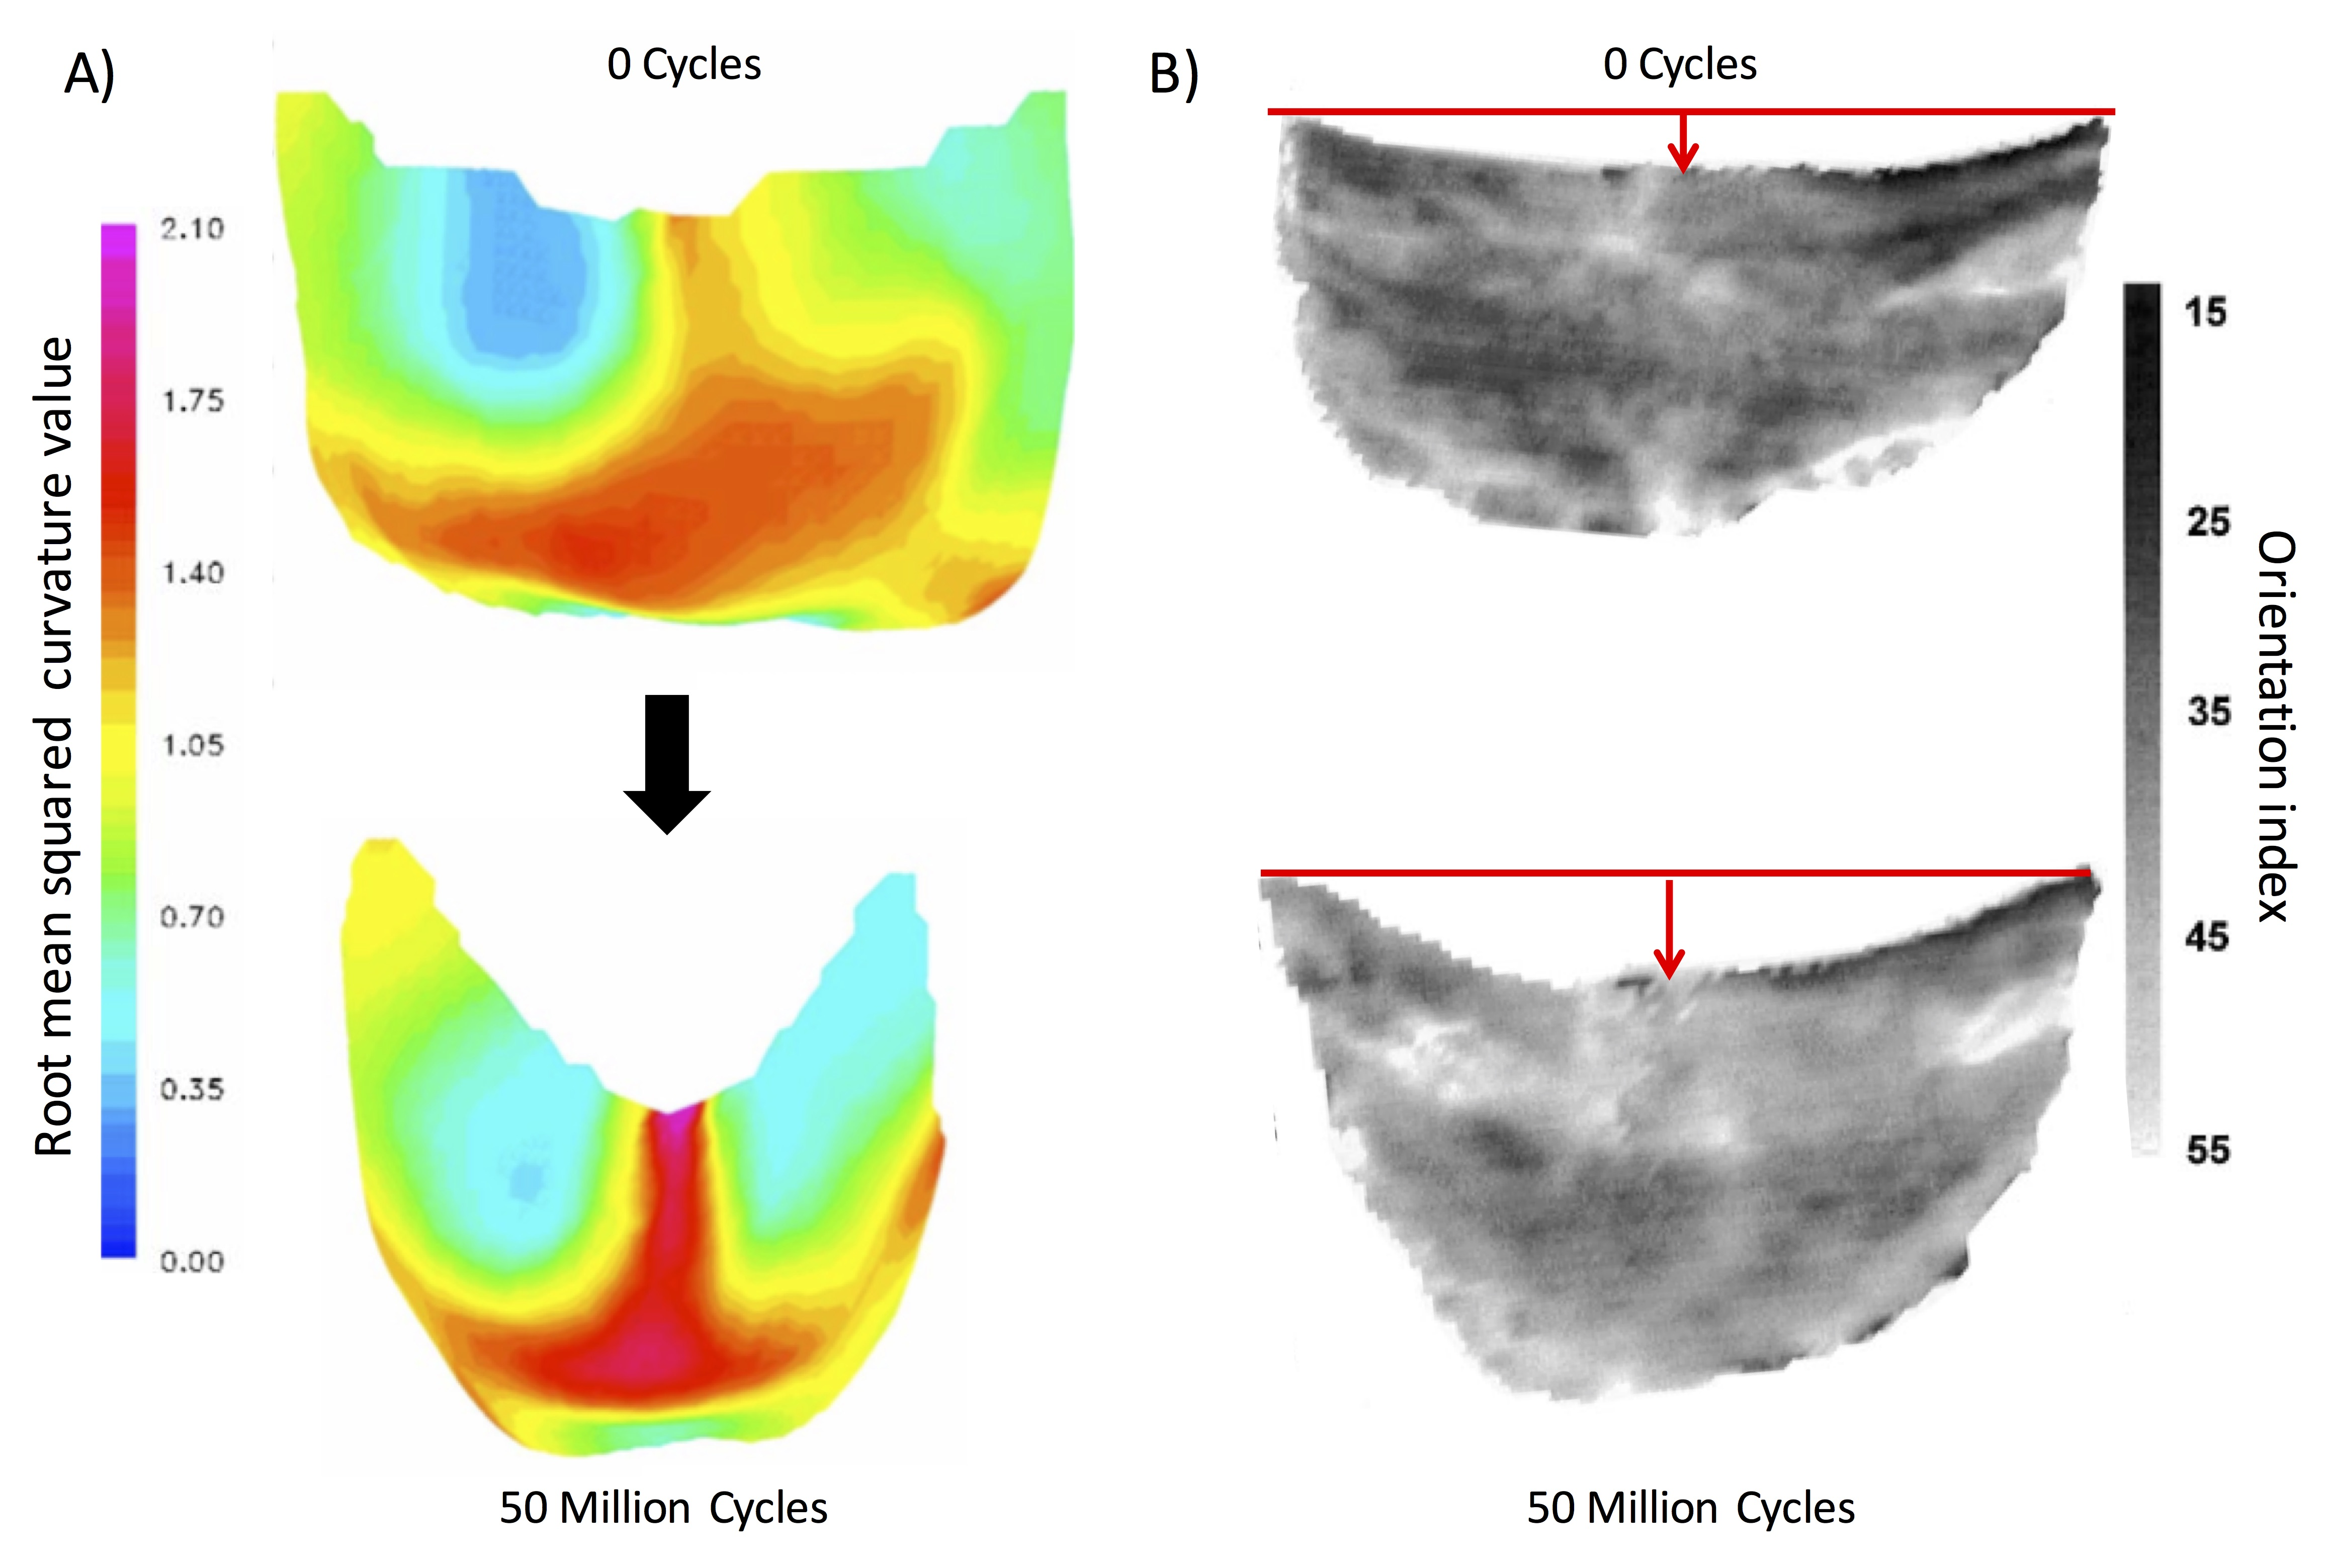
\includegraphics[width=0.55\paperwidth]{Images/chapter4/figure1.jpg}
\caption{A) The 3D unloaded geometry a BHV leaflet before and after cyclic loading. The color shows the root mean squared curvature of the leaflet. The most significant change in geometry is in the belly region. B) Small angle light scattering imaging of the flattened BHV leaflet used to examine the collagen fiber architecture. The collagen fiber architecture are convected by the dimensional changes but the corresponding regions remain mostly the same.}
\label{fig:PSeffects}
\end{figure}





\subsection{The effect of exogenous crosslinking}

	Bovine pericardium (BP) is a dense collagenous tissue composed mostly of collagen type I fibers with some elastin, GAGs, cells and vasculature. 
	Collagen fibers are complex protein structures at the 2 - 10 $\mu$m scale, made from tightly bundled collagen fibrils. 
	Much of we know about the use of GLUT to exogenously crosslink collagenous tissue is from the previous works of Nimni \textit{et al.}\cite{cheung_mechanism_1990, nimni_chemically_1987, cheung_mechanism_1985, gendler_toxic_1984, cheung_presence_1983, cheung_mechanism_1982, cheung_mechanism_1982b}. 
	GLUT, which is an aldehyde based crosslinker, aggressively crosslinks free amines in proteins. 
	This suppresses immunogenicity by crosslinking all cell membrane protein remnants, but also form polymeric networks (at the nm scale) which allows for long range crosslinks to the nearby tissue microstructures. 
	We previously found that exogenous crosslinking increases the bending stiffness of the matrix by four time the original stiffness \cite{mirnajafi_effects_2010}.
	We also tested the mechanical response exogenously crosslinked BP before and after crosslinking, and developed the first constitutive model for exogenously crosslinked soft tissue \cite{sacks_novel_2016}. 
	Interestingly, we also found that exogenously crosslinking does not increase the collagen fiber modulus, but significantly increases the interactions between collagen fibers \cite{sacks_novel_2016}, which is responsible for up to 30\% of the stress in the fully loaded state. 


	GLUT crosslinking is a Schiff-base reaction, which are known for their unstable molecular bonds \cite{migneault_glutaraldehyde_2004, damink_glutaraldehyde_1995}. 
	Although highly reactive and readily form crosslinks, the crosslinks formed by GLUT also readily undergo hydrolysis \cite{migneault_glutaraldehyde_2004}, allowing for the scission-healing of the GLUT polymer network to occur continuously at body temperature. 
	Under cyclic loading, this re-crosslinking occurs continuously and allow for the exogenously crosslinked matrix to gradually change in reference configuration to the current loaded state. 
	\emph{We hypothesize that this scission-healing behavior could be linked to the  mechanisms that underlie the changes in BHV geometry over time}. 
	
	
This non-damage related change in the BHV geometry has many similarities to the permanent set (PS) mechanisms observed in elastomers. 
Permanent set is an irreversible deformation that remains in a structure or material after it has been subjected to stress. 
It does not induce any damage to the constituents of the material, but instead changes the referential configuration. 
Although the outcomes may be similar, permanent set is not a plastic deformation as deformations are entirely in the elastic regime of the material. 
In particular, it is used to model the scission-healing reaction of elastomers that occurs when heated. 
Here, elastomers are stretched, heated, cooled, then unloaded, allowing some of the materials to change in referential configuration to the loaded state. 
In this process, permanent set does not damage the polymeric fibers but is a result of the change in configuration of the underlying polymeric fiber network. 
Some works on constitutive models of this process include the works of Rajagopal and Wineman\cite{rajagopal_constitutive_1992}, Andrews and Tobolsky\cite{andrews_theory_1946}, and Rottach \textit{et al}.\cite{rottach_effect_2004, rottach_molecular_2007, rottach_permanent_2006}. 
However, there are no known studies on the permanent set effect in soft tissues or soft tissue derived biomaterials. 
	

	\emph{Based on known considerations, we hypothesize that the initial time evolving BHV geometry and mechanical response can be predicted by permanent set mechanisms.} 
	Rather than heating and cooling, we assume that permanent set in exogenously crosslinked tissue occurs continuously at body temperature due to the GLUT, allowing the reference configuration of the exogenously crosslinked matrix to evolve over time. 
	As a result, the reference configuration of BHVs will change while not affecting the intrinsic material properties of their constituents such as collagen fibers and the exogenously crosslinked matrix. 
	Since the BHVs deform into a new configuration (Fig. \ref{fig:PSeffects}), there may develop regions of stress concentrations. 
	The high stresses will increase the rate of structural damage and thus accelerate the rate of BHV failure. 
	Thus, \emph{by compensating for the permanent set effects, it may be possible to reduce the BHV leaflet stresses and thus reduce structural damage to BHVs during \textit{in vivo} operation after implant.} 
	Therefore, constitutive models that can predict the effects of permanent set are crucial for the simulation of BHVs. 
		

\subsection{Constitutive models for the permanent set effect for soft tissues}

	There has been very little research in the constitutive modeling and simulation of the permanent set effect in native or exogenously crosslinked soft tissues. 
	The only work in this area is the pioneering study of Martin and Sun \cite{martin_modeling_2013}, who developed a time dependent constitutive model for uniaxial cyclic loading of GLUT exogenously crosslinked BP strips using a damage analog. 
	Briefly, to model the uncycled mechanical response, they used the Fung hyperelastic model for the strain energy density function, $\Psi_0$. 
	The time dependent stress softening was then described using a modification to the strain energy function as $\Psi_\mathrm{PS} = (1-D_s)\Psi_0 - \Psi_0(\mathbf{E}_\mathrm{PS})$. 
	Here the strain energy of the material after permanent set ($\Psi_\mathrm{PS}$) is reduced from $\Psi_0$ in accordance with a scaled damage function $D_s$ and the same strain energy function evaluated at the current amount of permanent set ($\mathbf{E}_\mathrm{PS}$). 
	Martin and Sun then measured the maximum permanent set deformation that occurs for each specimen, and used that to set the maximum bound of $\mathbf{E}_\mathrm{PS}$. 
	Additionally, Martin and Sun set two parameters, a lowerbound below which no permanent set occurs, and an upperbound above which the tissue fails. 
	In the intermediate region, $D_s$ and $\mathbf{E}_\mathrm{PS}$ simply increases linearly with the number of cycles. 
	The number of cycles needed to reach the maximum permanent set deformation was then described using an inverse exponential like function of the maximum strain applied, which is an analogous to the stress versus cycles (S–N) curve used to describe the fatigue behavior of traditional engineering materials.
	However, such approaches have the following limitations: 
	1) they are not predictive as there are no underlying mechanisms in the model. 
	A damage-like model can mimic the results of permanent set but cannot explain the mechanisms responsible in exogenously crosslinked tissue, and 2) there is no way to extend it for predicting into unmeasured regimes using the Fung hyperelastic model. 
	Therefore, there is a need for a more predictive constitutive model that utilizes the underlying mechanisms.

	

\subsection{A new approach for modeling the permanent set effect in exogenously crosslinked soft tissues}

	We utilize structural constitutive models, which integrate information on tissue composition and structure for material characterization \cite{sacks_structural_2000}. 
	In principal, using structural models, we only need to do parameter estimation for the innate material properties such as collagen fiber modulus and matrix modulus, and then use the microstructure of the tissue to predict the mechanical response \cite{zhang_meso_2016, fata_insights_2014}. 
	As a result, structural models have the potential to predict the mechanical response when extrapolating past the range of the experiment data.
	Thus, by using a structural modeling approach, we can use 1) the uncycled mechanical response of the BHV leaflet tissue and 2) the mechanisms responsible for the evolving leaflet microstructure due to permanent set to predict the evolving mechanical response of the BHV leaflet. The key aspects of our approach include:
\begin{enumerate}
\item Model the change in mechanical response entirely as a kinematic change in the underlying microstructure; no actual change in mechanical properties (damage)
\item Predict the change in geometry from the loading history and the permanent set mechanism
\item Validate the permanent set mechanism under both strain and stress controlled loading conditions
\item Develop a time dependent implementation with an evolving loaded configuration under stress control
\end{enumerate}